%%%%%%%%%%%%%%%%%%%%%%%%%%%%%%%%%%%%%%%%%%%%%%%%%%%%%%%%%%%%%%%%%%%%%%%%%%%%%%%%%%%%%%%%%
%%                                                                                     %%
%%                This file is part of the CAPH Compiler distribution                  %%
%%                            http:%/caph.univ-bpclermont.fr                           %%
%%                                                                                     %%
%%                                  Jocelyn SEROT                                      %%
%%                         Jocelyn.Serot@univ-bpclermont.fr                            %%
%%                                                                                     %%
%%         Copyright 2011-2018 Jocelyn SEROT.  All rights reserved.                    %%
%%  This file is distributed under the terms of the GNU Library General Public License %%
%%      with the special exception on linking described in file ..%LICENSE.            %%
%%                                                                                     %%
%%%%%%%%%%%%%%%%%%%%%%%%%%%%%%%%%%%%%%%%%%%%%%%%%%%%%%%%%%%%%%%%%%%%%%%%%%%%%%%%%%%%%%%%%

\chapter{Model of Computation} \label{cha:moc}

In this chapter, we describe a \emph{model of computation} (MoC) which can be used to describe the
behavior of CAPH programs. The goal is threefold.

\medskip
First is to place CAPH on the ``map'' of dataflow-based formalisms and languages, which is generally
organized in terms of associated MoCs (KPN, DPN, SDF, CSDF, \ldots), for the sake of comparison and
communication. 

Second is to give a formal description of the behavior of CAPH programs at a higher level than
that provided by the structural operational semantics rules given in
chapter~\ref{chap:dynamic-semantics}. 

Third is a to settle the basis for a mechanism allowing (when applicable) the static computation of FIFO
  sizes.

\medskip
The CAPH MoC is a variant of the \emph{Dataflow Process Network} model. We  therefore start by
recalling the main features of the DPN model, in Sec.~\ref{sec:dpn}. The CAPH MoC is presented in
this context in Sec.~\ref{sec:caph-moc}. In Sec.~\ref{sec:stat-comp-fifo} we discuss the application
of this model to the third of the objectives listed above, namely the prediction of FIFO sizes.


\section{Dataflow Process Networks}
\label{sec:dpn}

The \emph{Dataflow Process Network} (DPN) model has been introduced and formalized by Lee and Parks
in~\cite{DPN}. It can be viewed as a generalization of the \emph{Kahn Process
  Network} model introduced by Kahn in~\cite{Kahn74}. The presentation of the DPN model in this
section is directly inspired by that given in~\cite{DPN}, with slight variations in the notations
in order to ease the derivation of the CAPH MoC from it.

\medskip
In the DPN model, a program is a collection of processes communicating through unidirectional, unbounded
FIFO channels. Both read and write from/to these channels are unblocking\footnote{This is the main
  distinction with the KPN model, where write is unblocking but read is always blocking.}. Each
FIFO channel carries a sequence of \emph{tokens} and each process consists of repeated
\emph{firings} of a dataflow \emph{actor}. Each firing can read (and possibly consumes) tokens on
the channels connected to the input ports and can write (produce) tokens on the output ports of the
corresponding actor.

\medskip
\noindent
In the DPN model, each token carries a \textbf{value} $x$ taken from an uninterpreted \textbf{domain} $D$.

\medskip
\noindent
Channels contains (ordered, finite or infinite) \textbf{sequences} of tokens. A sequence will be
denoted

\begin{center}
  \begin{math}
    X = [x_1, x_2, \ldots]   \qquad \text{where} \quad x_i \in D \quad \forall i
  \end{math}
\end{center}

\medskip
\noindent
We will write $[]$ for the empty sequence and denote $\sqsubseteq$ the classical \textbf{prefix} ordering relation between
sequences. For example

\begin{eqnarray*}
    [x_1,x_2] & \sqsubseteq & [x_1,x_2,x_3]
\end{eqnarray*}

and

\begin{eqnarray*}
    [] & \sqsubseteq & [x_1]
\end{eqnarray*}

\medskip
\noindent
The behavior of an actor with $m$ input ports and $m'$ output ports is the defined by a set
$\mathcal{R}$ of $N$ \textbf{firing rules}

\begin{eqnarray*}
  \mathcal{R} & = & \{ R_1, R_2, \ldots, R_N \}
\end{eqnarray*}

where each firing rule $R_i$ is defined as a set of $m$ \textbf{rule input patterns} and $m'$ \textbf{rule
output patterns}

\begin{eqnarray*}
  R_i & = & \{ R_{i,1}, R_{i,1}, \ldots, R_{i,m},\ R'_{i,1}, R'_{i,1}, \ldots, R'_{i,m'} \}
\end{eqnarray*}

\medskip
\noindent
A \textbf{rule input pattern} is a (finite, possibly empty) sequence of \textbf{input patterns} 

\begin{eqnarray*}
  R_{i,j} & = & [ p_1, p_2, \ldots, p_n ] \quad (j \in \{1,\ldots,m\},\ n \geq 0)
\end{eqnarray*}

where a \textbf{input pattern} $p$ is either
\begin{itemize}
\item a \emph{constant value} $x \in D$,
\item the \emph{wildcard} pattern $*$.
\end{itemize}

\medskip
\noindent
A \textbf{rule output pattern} is a (finite, possibly empty) sequence of wildcard
patterns\footnote{A rule output pattern then simply indicates  \emph{how many} of tokens produced
  on a given output port when the corresponding rule is fired, regardless of the actual values
  carried by these tokens.} 

\begin{eqnarray*}
  R'_{i,j} & = & [ *_1, *_2, \ldots, *_{n'} ] \quad (j \in \{1,\ldots,m\},\ n' \geq 0)
\end{eqnarray*}

\medskip
\noindent
The \textbf{context} of a process is a, ordered set composed of the input sequences $\{X_1,\ldots,X_m\}$
present on the $m$ channels connected to the input of this actor.

\medskip
\noindent
A rule $R_i$ is said to be \textbf{fireable} in a context $C=\{X_1,\ldots,X_m\}$ if and only if

\begin{center}
  \begin{math}
    \forall j=1,\ldots,m \quad R_{i,j} \models_r X_j
  \end{math}
\end{center}

where $\models_r$ is the relation indicating whether a given input
sequence $X_j$ ``matches'' the corresponding rule pattern $R_{i,j}$. This relation can be defined
recursively as follows, using ``\verb|:|'' as the sequence concatenation
operator\footnote{$x_1 : [x_2,x_3,\ldots] = [x_1,x_2,x_3,\ldots]$.} : 
\begin{eqnarray*}
    []  & \models_r & X  \qquad \forall X \\
    p:ps & \models_r & x:xs \qquad \text{iff}\quad p \models_p x \quad \text{and}\quad ps \models xs
\end{eqnarray*}

and where the \textbf{pattern matching relation} $\models_p$ is defined as follows :
\begin{eqnarray*}
* & \models_p & x \qquad \forall x \in D \\
x & \models_p & x' \qquad \text{iff}\quad x=x'
\end{eqnarray*}

\medskip
\noindent
As an example, consider an actor with $m=3$ inputs and $m'=2$ outputs and the following firing rule

\begin{eqnarray*}
    R_1 & = & \{ [*,*], [], [1],\ [*], [*,*] \}
\end{eqnarray*}

\noindent
This rule will be fireable in any context $C=\{X_1,X_2,X_3\}$ in which
\begin{itemize}
\item $X_1$ contains at least two unconsummed tokens (regardless of their value),
\item $X_3$ contains at least one token with value equals to 1,
\item $X_2$ contains any sequence (possibly, but not necessarily, empty).
\end{itemize}
\noindent
and, when fired, it produces one token on the first output port and two tokens on the second.

\medskip
\noindent
An actor is said to be \textbf{fireable} in a given context if at least one of its rules is
fireable. If, in any case, \emph{at most} one rule is fireable, the actor is said to be
\textbf{deterministic}.

\medskip
\noindent
A classical example of a DPN actor is that described in Fig.~\ref{fig:select-dpn}. This actor reads
a token carrying a boolean value on its third input and, depending on this value, copy the token
present on its first or second input to its output. The behavior of the \texttt{select} actor can be
described by a set of two firing rules $\{R_1, R_2\}$ where

\begin{eqnarray*}
  R_1 & = & \{ [*], [], [\mathsf{true}],\ [*] \} \\
  R_2 & = & \{ [], [*], [\mathsf{false}],\ [*] \}
\end{eqnarray*}

\begin{figure}[h]
  \centering
  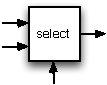
\includegraphics[width=3cm]{figs/select-dpn}
  \caption{The \texttt{select} actor}
  \label{fig:select-dpn}
\end{figure}

\medskip
\noindent
The \textbf{signature} $|R_i|$ of a firing rule $R_i$ gives the number of tokens consummed on each input
channel and produced on each output channel when the rule is fired :

\begin{eqnarray*}
  | R_i | & = & \{ |R_{i_1}|, \ldots, |R_{i,m}|,\ |R'_{i_1}|, \ldots, |R'_{i,m'}| \}
\end{eqnarray*}

where the ``length'' of the rule pattern $R_{i,j}$ is defined as 

\begin{eqnarray*}
  |R_{i,j}| & = & |\{p_{i,j,1},\ldots,p_{i,j,n}\}| \\
           & = & n
\end{eqnarray*}

\medskip
\noindent
For example, for the \texttt{select} actor introduced above, we have
\begin{eqnarray*}
  |R_1| & = & \{1, 0, 1,\ 1\} \\
  |R_2| & = & \{0, 1, 1,\ 1\}
\end{eqnarray*}

\bigskip
\noindent
The set of rule signatures can be used to refine the model of computation of an actor. For example,
an actor which consumes (resp. produces) a fixed number of tokens on each input (resp. output) at each activation, \ie an actor for
which

\begin{eqnarray*}
  |R_i| & = & \{ k_1, \ldots, k_m,\ k'_1, \ldots, k'_{m'} \} \qquad \forall i=1,\ldots,N
\end{eqnarray*}

is categorized as belonging to \textbf{SDF} (Synchronous Dataflow) model of computation.

\section{The Caph Process Network model}
\label{sec:caph-moc}

The model of computation for CAPH -- let's call it CPN, for \emph{Caph Process Network} -- can be
viewed as a variant of the DPN model summarized in the previous section. The variations concern the
type of values carried by tokens on the one hand and the form of the patterns used to define the
firing rules on the other hand.

\subsection{Token values}
\label{cpn-token-value}

\newcommand{\mocatom}{\mathsf{a}}
\newcommand{\mocvar}{\mathsf{v}}
\newcommand{\mocconst}{\mathsf{c}}
\newcommand{\moctuple}{(\mocatom_1,\ldots,\mocatom_n)}
\newcommand{\moccon}{\chi\ (\mocatom_1,\ldots,\mocatom_n)}

The set of values carried by tokens is obtained by enriching the basic domain $D$ used in the DPN
model with two types of \emph{structured} values :
\begin{itemize}
\item tuples of atomic values, denoted $(x_1,\ldots,x_n)$ (where $n \geq 1$ and $x_i$ are atomic values),
\item constructed values, of the form $\chi\ (x_1,\ldots,x_n)$ where $n \geq 1$, $\chi$ is a $n$-ary
  value constructor (taken from a predefined set of constructors $\mathsf{Con}$) and the $x_i$s are
  atomic values.
\end{itemize}
Formally, we therefore define the domain $D$ of token values in the CPN model as
\begin{eqnarray*}
  D & := & \mocatom \qquad \text{atomic value (int, bool, \ldots)} \\
    & |  & \moctuple \qquad \text{(tuples)} \\
    & |  & \moccon \qquad \text{where}\ \chi \in \mathsf{Con} \qquad (\text{constructed values)}
\end{eqnarray*}

\subsection{Rule patterns}
\label{cpn-rpatterns}

In the CPN model, rule patterns cannot have a length $\ge 1$ :

\begin{eqnarray*}
  \forall i=1,\ldots,N, & \forall j=1,\ldots,m  &|R_{i,j}| \in \{0,1\} \\
                        & \forall j=1,\ldots,m'  &|R'_{i,j}| \in \{0,1\}
\end{eqnarray*}

\medskip
\noindent
In other words, deciding whether a given rule is fireable can only involve the \emph{first} token
present of each input sequence and the activation of a rule can produce at most one token of each
output. The main reason for this is that it allows hardware implementations
to rely on a simple, fixed-interface FIFO model\footnote{Allowing an actor to read -- and \emph{a
    fortiori} ``pop'' -- $n>1$ tokens from a FIFO requires a significantly more complex interface,
  especially if $n$ cannot be computed statically.}. Moreover, our experience, based upon a large
set of realistic applications, showed that this restriction does not in practice limit the
expressiveness of the language.

\subsection{Patterns}
\label{cpn-patterns}

The set of individual patterns is augmented to accomodate the new definition of the domain $D$ for
values :
\begin{eqnarray*}
  p & := & * \qquad (\text{wildcard pattern}) \\
    & |  &  c \in D \qquad \text{(constant pattern)} \\
    & |  & v \in \mathsf{Var} \qquad \text{(variable pattern)} \\
    & |  & (p_1,\ldots,p_n) \qquad \text{(tuple pattern)} \\
    & |  & \chi\ (p_1,\ldots,p_n) \qquad \text{(constructed pattern)}
\end{eqnarray*}

\medskip
\noindent
Variable patterns are used to \emph{bind} values associated to tokens to names in order to use them
in for constructing the outputs of a given rule. 

\subsection{Pattern matching}
\label{cpn-pattern-match}

The pattern matching relation $\models_p$ defined in Sec.~\ref{sec:dpn} is modified as follows
to take account the previous modifications :
\begin{eqnarray*}
* & \models_p & \mocatom \qquad \forall \mocatom \\
c & \models_p & \mocatom \qquad \text{iff}\quad x=\mocatom\\
v & \models_p & \mocatom \qquad \forall \mocatom \\
(p_1,\ldots,p_n) & \models_p & \moctuple \qquad \text{iff}\quad p_i \models_p \mocatom_i \quad \forall j=1,\ldots,n \\
\chi'\ (p_1,\ldots,p_n) & \models_p & \moccon \qquad \text{iff}\quad \chi = \chi' \quad \text{and} \quad p_i \models_p \mocatom_i \quad \forall j=1,\ldots,n 
\end{eqnarray*}

\subsection{Example}
\label{cpn-example}

Figure~\ref{fig:cpn-ex1} shows an actor defined in CAPH and the three firing rules defining the
behavior of this actor in the CPN model of computation.

\lstset{frame=none}
\begin{figure}[h]
  \centering
\begin{tabular}[c]{cc}
  \begin{minipage}{0.5\textwidth}
\begin{lstlisting}
type opt = None | Some of int;

actor foo
  in (i1: opt, i2: int)
  out (o:int)
rules 
  | (i1: Some x) -> x
  | (i1: None, i2:0) -> 1 
  | (i1: None, i2:y) -> y
;
\end{lstlisting}
  \end{minipage} &
  \begin{minipage}{0.5\textwidth}
\begin{eqnarray*}
  R_1 & = & \{[\mathsf{Some}\ x], [],\ [*]\} \\
  R_2 & = & \{[\mathsf{None}, [0],\ [*]\} \\
  R_3 & = & \{[\mathsf{None}, [y],\ [*]\}
\end{eqnarray*}
  \end{minipage}
\end{tabular}
  \caption{A CAPH actor and the associated firing rules in the corresponding model of computation}
  \label{fig:cpn-ex1}
\end{figure}
\lstset{frame=single}

\subsection{Classification of CAPH actors}
\label{sec:class-caph-actors}

The rule signatures of an actor can be used to classify the behavior of this actor into three
categories : SDF, CSDF and DDF.

\subsubsection{SDF Actors}
\label{sec:sdf-actors}

SDF (Synchronous Data Flow) actor are those for which all firing rules have the same signature

\begin{eqnarray*}
|R_i| & = & \{ \rho_1, \ldots, \rho_m,\ \rho'_1, \ldots, \rho'_{m'} \}   \qquad \forall i=1,\ldots,N
\end{eqnarray*}

The CAPH model of computation imposes that $\rho_j \in \{0,1\}\ \forall j=1,\ldots,m$ and $\rho'_j
\in \{0,1\}\ \forall j=1,\ldots,m'$. But for an SDF actor, having $\rho_j = 0$ (resp. $\rho'_j=0$)
would mean that this actor \emph{never} consumes (resp. produces) a token on the $j^{th}$ input
(resp. output) channel. There's no loss in expressivity in excluding this type of behaviors. As a
result, SDF actors in CAPH are those for which all firing rules have a signature

\begin{eqnarray*}
  |R_i| & = & \{1, \ldots, 1,\ 1, \ldots, 1\}
\end{eqnarray*}

\medskip Listings~\ref{lst:add-act} and \ref{lst:scale-act} give two examples of actors which can
classified as SDF. The \verb|add| actor operates (here) on unstructured streams os signed integers
whereas the \verb|scale| actor operates on streams structured as lists using the \verb|dc|
type\footnote{The type \texttt{t dc} is a variant type. Values belonging to this type can be either
  the constant constructors \texttt{SoS} or \texttt{EoS} (\emph{Start of Structure} or \emph{End of
    Structure} or the constructed value
  \texttt{Data v}, where \texttt{v} has type \texttt{t}.}. For both
actors, each rule consumes and produces exactly one token when fired\footnote{The signature of the
  rules has been here indicated as a comment. In practice, it will be computed by the compiler.}. 

\begin{lstlisting}[caption={A simple SDF actor in CAPH},label=lst:add-act]
actor add 
  in (i1:signed<s>, i:signed<s>)
  out (o:signed<s>)
rules
| (i1:x1,i2:x2) -> o:x1+x2       -- Rule R1 ({1,1, 1})
;
\end{lstlisting}

\begin{lstlisting}[caption={Another SDF actor},label=lst:scale-act]
actor scale (k:unsigned<s>)
  in (i:unsigned<s> dc)
  out (o:unsigned<s> dc)
rules
| i:SoS -> o:SoS                  -- Rule R1 ({1, 1})
| i:Data(v) -> o:Data(v*k)        -- Rule R2 ({1, 1})
| i:EoS -> o:EoS                  -- Rule R3 ({1, 1})
;
\end{lstlisting}

\subsubsection{CSDF Actors}
\label{sec:csdf-actors}

For CSDF (Cyclo Static Data Flow) actors, several firing rules, with distinct signatures, coexist
but the order at which these rules are fired is statically predictable. The behavior of
such an actor can generally be described as a finite state machine whose transitions depend solely on the
value of local variables (and not on the value of tokens read on inputs).

\medskip
An example of actor which can be classified as CSDF is given is Listing~\ref{lst:switch-act}.
The \verb|switch| actor\footnote{This actor has already been described in
  Sec.~\ref{sec:actor-examples}.} reads tokens on
its input channel and alternatively routes them to its first (``left'') and second (``right'')
output. This is accomplished using the local variable \texttt{s}, which is alternately set
  to the (enumerated) values \texttt{Left} and \texttt{Right}.
Given the input stream
\begin{equation*}
x_1, x_2, x_3, x_4, x_5, x_6 \ldots  
\end{equation*}
it produces the following output streams on its first and second output
\begin{eqnarray*}
x_1, x_3, x_5, \ldots  \\
x_2, x_4, x_6, \ldots  
\end{eqnarray*}

\begin{lstlisting}[caption={A simple CSDF actor in CAPH},label=lst:switch-act]
actor switch
  in (i:$1)
  out (o1:$1, o2:$1)
  var s : {Left,Right} = Left
  rules
  | (s:Left, i:v) -> (o1:v, s:Right)  -- Rule R1
  | (s:Right, i:v) -> (o2:v, s:Left)  -- Rule R2
;
\end{lstlisting}
%$

The signature of the first and second rule are respectively $|R_1|=\{1,\ 1,0\}$ and
$|R_2|=\{1,\ 0,1\}$ but is should be clear from the definition of these rules that they fire
alternatively and cyclically as follows

\begin{equation*}
  R_1, R_2, R_1, R_2, R_1, \ldots
\end{equation*}

In fact, this property can be established formally
using a technique known as \emph{abstract interpretation}. Application of this technique to the
classification of dataflow actors has been described for example in~\cite{Wipliez2012}. It can here
prove that the only sequence of values that the local variable \verb|s| can take is

\begin{center}
\begin{verbatim}
Left, Right, Left, Right, ...
\end{verbatim}
\end{center}

\noindent
which is sufficient to prove that the rules fires in the aforementionned order.

% \lstset{frame=none}
% \begin{figure}
%   \centering
%   \begin{tabular}[t]{cc}
%     \begin{minipage}[c]{0.75\linewidth}
%       \begin{lstlisting}
% actor sample2
%   in (i:$t)
%   out (o:$t)
% var st: {S0,S1} = S0
% rules
% | (st:S0, i:x) -> st:S1         -- Rule R1 ({1,0})
% | (st:S1, i:x) -> (o:x, st:S0)  -- Rule R2 ({1,1})
% ;
%       \end{lstlisting}
%     \end{minipage}
% \adjustbox{valign=c}{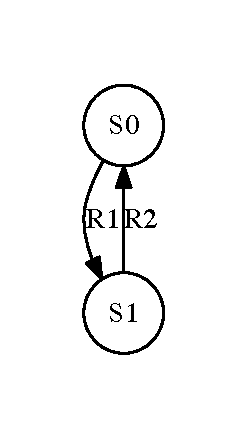
\includegraphics[width=0.2\textwidth]{figs/sample2-act}}
% % Source code & Associated FSM
%   \end{tabular}
%   \caption{A $2 \rightarrow 1$ subsampling actor}
%   \label{fig:cpn-ex2}
% \end{figure}
% \lstset{frame=single}

\medskip
Another example of CSDF actor is given in Listing~\ref{lst:cpn-ex3}. The \verb|sample|
actor\footnote{Which is taken from the CAPH standard library.} performs $n \rightarrow 1$
subsampling. Given the input stream
\begin{equation*}
x_1, x_2, x_3, x_4, x_5, x_6 \ldots  
\end{equation*}
it produces the output stream
\begin{equation*}
x_n, x_{2n}, x_{3n}, \ldots  
\end{equation*}

Using abstract interpretation, it is still possible to classify the \verb|sample| actor as CSDF, as
soon as the value of its parameter $n$ is known\footnote{This underlines a important distinction
  between the definition of an \emph{actor}, in which the behavior may depend on formal
  \emph{parameters} (such as \texttt{n} in the current example), and the actual \emph{instances} of
  this actor in the program graph (\emph{boxes} in the CAPH terminology), in which all parameters
  have been bound to values.}. For example, Fig.~\ref{fig:cpn-ex3b} gives the FSM obtained by
instanciating this actor with $n=4$, from which it is possible to predict this cyclic sequence of
consumption/production rates on \verb|(i,o)| : 

\begin{equation*}
  \{1,0\}, \{1,0\}, \{1,0\}, \{1,1\},\ \{1,0\}, \{1,0\}, \{1,0\}, \{1,1\},\ \ldots
\end{equation*}

\begin{lstlisting}[caption={A $n \rightarrow 1$ subsampling actor},label={lst:cpn-ex3}]
actor sample (n: int)
  in (i: $t)
  out (o: $t)
var k : {1,..,n} = 1
rules
| i:x when k<n -> k:k+1
| i:x when k=n -> (k:1, o:x)
;
\end{lstlisting}

\begin{figure}[h]
  \centering
  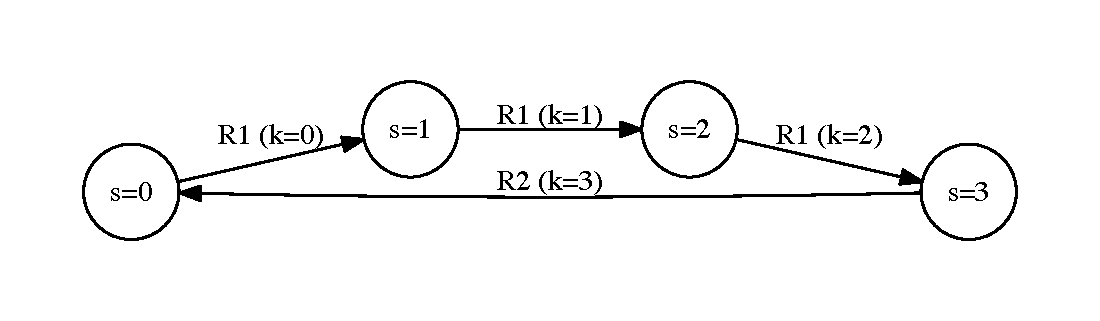
\includegraphics[width=0.75\textwidth]{figs/sample4-act}
  \caption{FSM for the \texttt{sample} actor with $n=4$}
  \label{fig:cpn-ex3b}
\end{figure}

\subsubsection{DDF Actors}
\label{sec:ddf-actors}

This category (Dynamic Data Flow) gathers all actors which cannot be classified as SDF or CSDF. 
For such actor it is not possible to statically predict the consumption/production rate on the I/O
channels because this rate ultimately depends on the \emph{value} of the tokens read by the actor. 

\medskip
\noindent
A first example of DDF actor is given in listing~\ref{lst:bswitch-act}. The \verb|bswitch| actor is
a variant of the \verb|switch| actor described in the previous section. It
routes the token read on its first input to either its first or second output depending on the
(boolean) \emph{value} of its second input. For example, given the following input streams on inputs \verb|i1| and \verb|i2| o
respectively
\begin{eqnarray*}
  0,        1,     2,    3,     4,    5, \ldots \\
  true, false, false, true, false, true, \ldots
\end{eqnarray*}
it will produce the output streams on the outputs \verb|o1| and \verb|o2|
\begin{eqnarray*}
  0, 3, 5, \ldots \\
  1, 2, 4, \ldots \\
\end{eqnarray*}
Because the selection of fired rule depends on the \emph{value} read on input \texttt{i2}, it is
not possible to statically decide which one will be selected and hence predict the production rate on
the outputs.

\begin{lstlisting}[caption={A simple DDF actor in CAPH},label=lst:bswitch-act]
actor bswitch
  in (i1:$t, i2:bool)
  out (o1:$t, o2:$t)
  rules
  | (i1:x, i2:true) -> o1:x      -- Rule R1 ({1,1, 1,0})
  | (i1:x, i2:false) -> o2:x     -- Rule R2 ({1,1, 0,1})
;
\end{lstlisting}
%$

\medskip
\noindent
A second, example of a DDF actor is described in listing~\ref{lst:suml-act2}. This
actor\footnote{Also previously described in Sec.~\ref{sec:actor-examples}.}
operates on a structured stream composed of a sequence of lists, each list starting with a
\verb|SoL| (\emph{StartOfList}) token and ending with a \verb|EoL| (\emph{EndOfList}) token. For each
list, it computes the sum of the elements.
For example, if

\begin{eqnarray*}
\mathtt{i} & = & \mathtt{SoL},\ 1,\ 2,\ 3,\ \mathtt{EoL},\ \mathtt{SoL},\ 4,\ 5,\ \mathtt{EoL},\ \ldots
\end{eqnarray*}

\noindent
then
\begin{eqnarray*}
\mathtt{o} & = & 6,\ 21,\ \ldots
\end{eqnarray*}

For this, it uses pattern
matching on the input to detect the start and end of each list and two local variables : a local
state (\texttt{state}), indicating whether the actor is waiting for a new list or computing the sum,
and a accumulator (\texttt{sum}) for computing the sum. The three transition rules can be read as
follows :
\begin{itemize}
\item if we are in state S0 and input token is ``\verb|SoL|'', then initialize sum to 0 and go to state S1;
\item if we are in state S1 and input token is a data, then add the corresponding value to the accumulator.
\item if we are in state S1 and input token is ``\verb|EoL|'', then writes the accumulated sum to output and
  go back to state S0;
\end{itemize}
This style of description, in which the \emph{size} of the processed data structures is neither
hard-coded nor provided using ``external'' parameters is actually very common in CAPH. It allows the
formulation of actors being able to operate on data structures (lists, images, \ldots) of \emph{any} size.

\begin{lstlisting}[caption={Another DDF actor},label=lst:suml-act2]
type $t list =
  SoL
| EoL
| Data of $t;

actor suml
  in (i:signed<16> list)
  out (o:signed<16>)
var state : { S0, S1 } = S0
var sum : int
rules 
| (state:S0, i:SoL)    -> (sum:0, state:S1)       -- Rule R1 ({1, 0})
| (state:S1, i:Data v) -> (sum:sum+v);            -- Rule R2 ({1, 0})
| (state:S1, i:EoL)    -> (o:sum, state:S0)       -- Rule R3 ({1, 1})
;
\end{lstlisting}

\medskip
As for the \verb|bswitch| actor, the exact sequence of rule firings cannot be predicted at compile
time. In fact, and provided that the input stream is well structured\footnote{I.e. that it is effectively constituted of successive
  lists, otherwise, the actor simply blocks.}, the sequence of firings can be described as 

\begin{equation*}
  \underbrace{\{1,0\},\ \{1,0\},\ \ldots,\ \{1,0\}}_{\text{n activations }},\ \{1,1\}
\end{equation*}

where $n$ depends on the actual length of the input lists and hence cannot be predicted.

\subsubsection{Implementation}
\label{sec:moc-class-impl}

A prototype implementation of MoC-based actor classification has been implemented in the CAPH
compiler since version 2.8.4. 

Classification is obtained by invoking the compiler with the \verb|-infer_mocs| option. Results are
written in a file named \verb|<prefix>_mocs.dat|, where \verb|<prefix>| is the name of the
application\footnote{As specified with the \texttt{-prefix} option or, by default, the current
  directory name.}. They can also be obtained with \verb|-dump_boxes| option. 

It is important to note that classification actually operates on \emph{boxes} and not on the actors
themselves. This is because this classification can depend on the actual value of actor
parameters, which are only known when actors are instanciated as boxes in the final process network.

\medskip
As an example, consider the program given in Fig.~\ref{fig:act-class-ex}. In this program, the
actors \verb|switch|, \verb|bswitch| and \verb|sample| are those introduced in the previous sections
and their code has not been reproduced. The \verb|merge| actor reads one token on each of its inputs
and alternatively writes that read on the first (resp. second) input to its output.

\lstset{frame=none}
\begin{figure}[h]
  \centering
\begin{tabular}[c]{cc}
  \begin{minipage}{0.5\textwidth}
\begin{lstlisting}[basicstyle=\small]
actor switch ... 

actor bswitch ...

actor sample (n: int) ...

actor merge 
  in (i1: $t, i2:$t)
  out (o:$t)
var st : {Left,Right} = Left
rules
| (st:Left, i1:x, i2:y) -> (o:x, st:Right)
| (st:Right, i1:x, i2:y) -> (o:y, st:Left)
;

stream i1:signed<8> from "sample1.txt";
stream i2:bool from "sample2.txt";
stream o1:signed<8> to "result1.txt";
stream o2:signed<8> to "result2.txt";

net (s1,s2) = switch i1;
net (s3,s4) = bswitch (s2,i2);
net o1 = sample 2 s1;
net s5 = sample 4 s3;
net o2 = merge (s5,s4);
\end{lstlisting}
%$
  \end{minipage} &
 \adjustbox{valign=c}{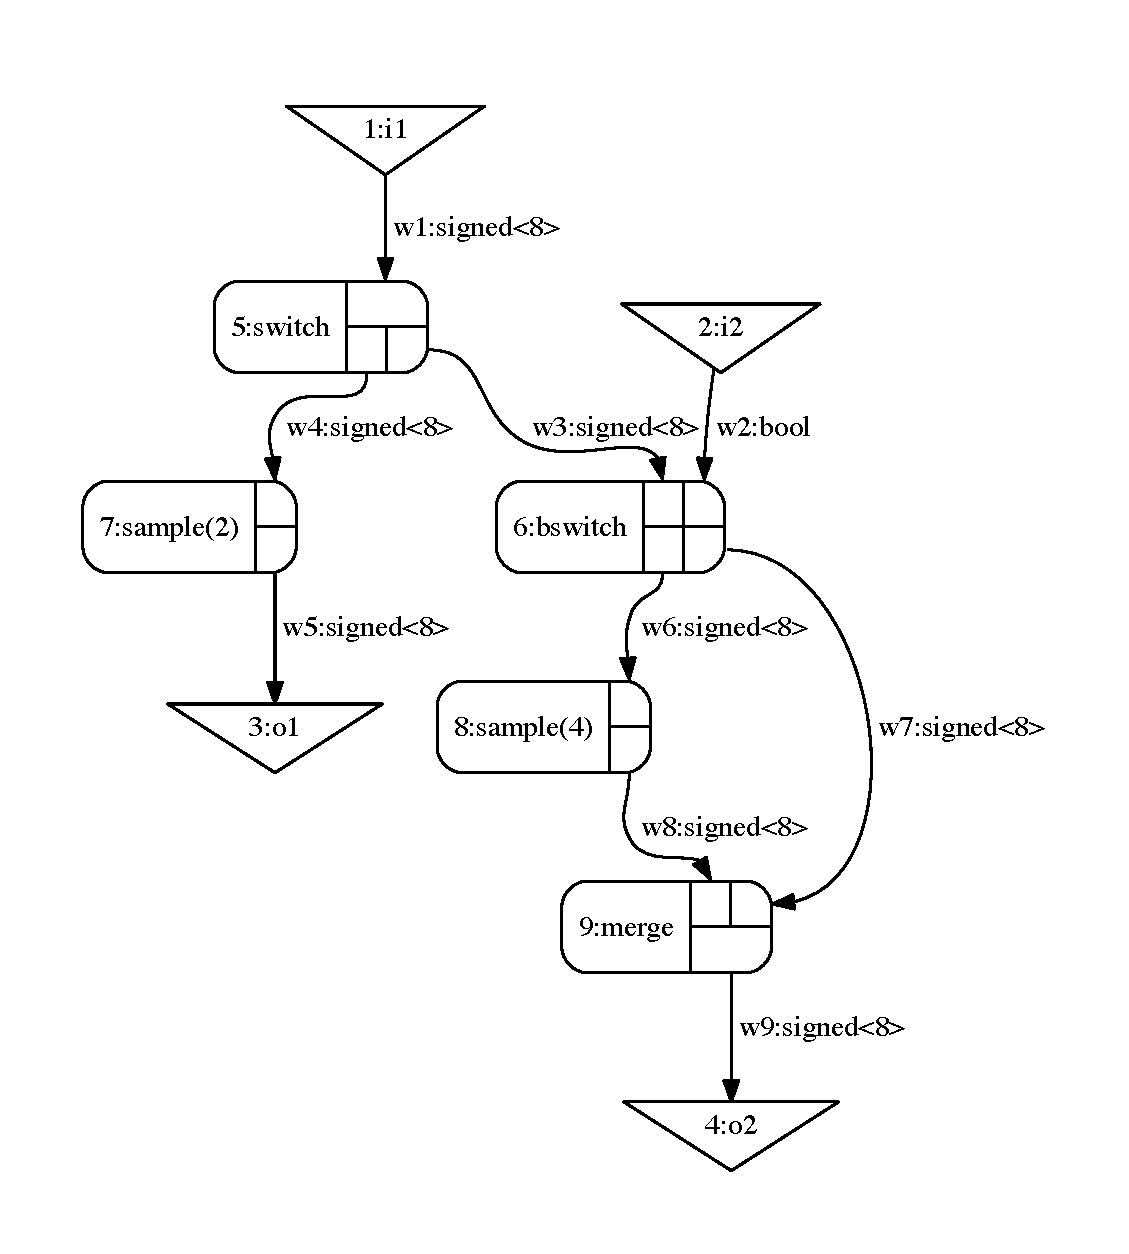
\includegraphics[width=0.5\textwidth]{figs/act-class-ex}}
\end{tabular}
  \caption{Example program for MoC-based actor classification}
  \label{fig:act-class-ex}
\end{figure}
\lstset{frame=single}


Classification is performed by invoking the compiler as follows (assuming that the program is
contained in file \verb|main.cph|, in directory \verb|test|) :

\begin{lstlisting}[language=bash]
caphc -infer_mocs main.cph
\end{lstlisting}

\noindent
This gives the following output 

\begin{lstlisting}[language=bash,basicstyle=\small]
This is the Caph compiler, version 2.8.4
...
> Running abstract interpreter on box B5(switch) to infer Moc... Done.
> Running abstract interpreter on box B6(bswitch) to infer Moc... Done.
> Running abstract interpreter on box B7(sample) to infer Moc... Done.
> Running abstract interpreter on box B8(sample) to infer Moc... Done.
Wrote file ./test_mocs.dat
\end{lstlisting}

The contents of the generated \verb|test_mocs.dat| file is given in Fig.~\ref{fig:act-class-res}. In
this listing 
\begin{itemize}
\item the first column gives the box identifier (as defined as a prefix number in the dataflow graph
  shown in Fig.~\ref{fig:act-class-ex}),
\item the second column gives the name of the instanciated actor,
\item the third column gives the name of the  infered MoC (\verb|sdf|, \verb|csdf| or \verb|ddf|),
\item the fourth column, in case of a \verb|sdf| (resp. \verb|csdf|) model, gives the box signature
  (resp. cyclic sequence of signatures).
\end{itemize}
This result shows that the compiler has correctly infered the model for each box. Note, in
particular, the difference in the infered sequence of signatures for the two instances of
the \verb|sample| actor (boxes \verb|B7| and \verb|B8|), due to the dependance of the activation
sequence on the value of the parameter \verb|n| of the actor.

\begin{figure}[H]
  \centering
\begin{verbatim}
B5; switch; csdf; [1,1,0],[1,0,1]
B6; bswitch; ddf
B7; sample; csdf; [1,0],[1,1]
B8; sample; csdf; [1,0],[1,0],[1,0],[1,1]
B9; merge; sdf; 1,1,1
\end{verbatim}
  \caption{Result of MoC-based box classification for the program of Fig.~\ref{fig:act-class-ex}}
  \label{fig:act-class-res}
\end{figure}

As evidenced by the compiler output reproduced above, classification was here obtained 
using \emph{abstract interpretation}.

The abstract interpreter used for MoC-based classification is based upon a modified version of
the dynamic semantics described in chapter~\ref{chap:dynamic-semantics}, in which a special value 
(typically noted $\bot$) is used to represent values which cannot be statically evaluated (such
the values carried by input tokens for instance). The interpreter iteratively fires the analysed box 
until one of the following conditions is met~:
  \begin{enumerate}
  \item an execution cycle is detected (in other words, the value of all known local variables is
    the same as it was at the first activation),
%   \item no more rule is fireable,
  \item the number of firings exceeds a given predefined limit.
  \end{enumerate}
The first condition is the one occuring for SDF for CSDF actors. The second condition is used to
detect DDF actors (with the assumption that CSDF actors generally have ``short'' periods and, hence,
that a sufficiently large value for the limit will be discriminant).  

It is possible to trace the execution of the abstract interpreter by inkoking the compiler with the
\verb|-absint| option with the identifier of the target box as argument\footnote{A complementary
  option, \texttt{ai\_max\_cycles}, serves to adjust the limit used to detect DDF actors.}. For our example, invoking the
compiler as follows

\begin{lstlisting}[language=bash]
caphc -infer_mocs -absint 8 main.cph
\end{lstlisting}

\noindent
gives the following output 

\begin{lstlisting}[language=bash,basicstyle=\small]
This is the Caph compiler, version 2.8.4
...
> abstract interpretation of box B8(sample) ...
> cycle detected at t=4:
>   [k=1] i:x, k<n -> k:k+1 [1,0]
>   [k=2] i:x, k<n -> k:k+1 [1,0]
>   [k=3] i:x, k<n -> k:k+1 [1,0]
>   [k=4] i:x, k=n -> k:1, o:x [1,1]
> done
\end{lstlisting}

This trace shows how the classification of box \verb|B8| as CSDF here results from the detection of
a cycle (of length 4) in the sequence of rule activations.

\subsection{Static computation of FIFO sizes}
\label{sec:stat-comp-fifo}

% Classifying actors into SDF, CSDF and DDF can be used to establish a kind of ``hierarchy'' between
% them. SDF actors have a very predictable but this comes at the expense of limited expressivity. By
% contrast, DDF actors are very expressive (it can be shown that they form a Turing-complete language)
% but predictability is limited. 

A potential application of actor classification can be the static computation of FIFO sizes.

Predicting the size (depth) of the FIFOs implementing the channels connecting actors is important
because an underestimation of these sizes may lead to runtime failure by overflow. When generating
VHDL code, overestimations also lead to a waste of hardware resources.

As described in Sec.~\ref{sec:adjusting-fifo-size}, this prediction is typically carried out using
runtime monitoring of the code generated by the SystemC backend. This approach may be the only
applicable for some programs involving actors with DDF behaviors. It is intuitively clear that the
size of the required FIFOs depends on the consumption and production rates of connected actors. If
these rates depend on the \emph{values} carried by tokens, so do the size of the FIFOs.

But not all programs involve DDF actors. For programs involving only SDF actors -- and, to a certain
extent\footnote{Which remains to be investigated\ldots}, CSDF actors --, it is possible to
accurately predict these sizes on the basis of a purely static analysis.

This is described, for SDF graphs, in the next section.

\subsubsection{SDF graphs}
\label{sec:sdf-fifo-sizing}

It is well known (see for example~\cite{Parks1995}) that for ``pure'' acyclic SDF graphs -- \ie
graphs for which all actors can be classified as SDF and exhibiting to feedback loops -- the size of
the buffers implementing channels can be statically computed. The basic technique relies on solving
the so-called \emph{balance equations}, relating production and consumption rates on extremities of
all edges.

\medskip In the case of CAPH programs, for which all production and consumption rates are equal to
1, these sizes can be computed in a more straigthforward way using the algorithm described below.
The algorithm basically works by propagating \emph{phases} along all edges of the dataflow graph, where
the phase ($\phi$) measures the propagation time (counted in execution cycles) of the input
token(s).  For a box to fire, each input edge must have the same phase. Otherwise, a FIFO must be
inserted on the ``late'' edge(s). The required FIFO capacity ($cap$) can be computed from the difference of
phases. Moreover, the phase of the output edge(s) can be simply computed by adding a constant
(representing the actor delay, in execution cycles) to the latest input phase.  

\begin{algorithm} \caption{Compute FIFO sizes of DFG G}
\label{alg:phase-prop}
\begin{algorithmic}[1]
\Require Each node n of G has been classified as SDF
\Ensure Each edge e of G is assigned a phase $\phi$ and a required FIFO capacity $cap$
\ForEach {$n \in SourceNodes(G)$}
\ForEach {$e \in v.outps$}
\State $e.\phi \gets 0$
\EndFor
\EndFor
\State $N \gets TopologicalSort(G)$
\While {$N \text{not empty}$}
\State $n \gets ExtractFirst(N)$
\State $\phi_m \gets max_{e \in n.ins}(e.\phi)$
\ForEach {$e \in n.ins$}
\If {$e.\phi < \phi_m$}
\State $e.cap \gets 1 + \phi_m - e.\phi$
\Else
\State $e.cap \gets 1$
\EndIf
\EndFor
\ForEach {$e \in n.outs$}
\State {$e.\phi \gets \phi_m + n.delay$}
\EndFor
\EndWhile
\end{algorithmic}
\end{algorithm}

\subsubsection{Implementation}
\label{sec:moc-class-impl}

A prototype implementation of the mechanism described in the previous section is available in
version 2.8.4 of the compiler.
This implementation generates an annotation file similar to that produced by the SystemC backend
used with the \verb|sc_dump_fifo_stats| (as described in Sec.~\ref{sec:adjusting-fifo-size} of the manual). 
This file can passed directly as argument to the \verb|vhdl_annot_file| option when invoking the
VHDL backend in order to specify the size of each hardware FIFO.

\medskip
The mechanism is invoked by passing the \verb|-dump_sdf_fifo_sizes| option to the compiler. Of
course, a necessary condition is that all boxes can be classified as SDF\footnote{Classification is
  performed as a preliminary step without the need to explicitely pass the
  \texttt{-infer\_mocs} option.}. 

\medskip 
As an example consider the program given in Listing~\ref{lst:sdf-fifosizes-ex}. The actual
computations performed by actors is irrelevant here, only their SDF signature is. 

\begin{lstlisting}[label=lst:sdf-fifosizes-ex,basicstyle=\small]
actor foo
  in (i:signed<8>)
  out (o:signed<8>)
rules
|  i:x -> o:x
;

actor bar
  in (i1:signed<8>, i2:signed<8>)
  out (o:signed<8>)
rules
|  (i1:x1, i2:x2)-> o:x1+x2
;

actor zib
  in (i:signed<8>)
  out (o1:signed<8>, o2:signed<8>)
rules
|  i:x-> (o1:x, o2:x)
;

stream inp:signed<8> from "sample.txt";
stream outp:signed<8> to "result.txt";

net (x2,x3) = zib inp;
net outp = bar (foo inp, bar (foo x2, foo (foo x3)));
\end{lstlisting}


Computing the FIFO sizes is performed by invoking the compiler as follows (assuming that the program is
contained in file \verb|main.cph|, in directory \verb|test|) :

\begin{lstlisting}[language=bash]
caphc -dot -dump_sdf_fifo_sizes main.cph
\end{lstlisting}

\noindent
This gives the following output 

\begin{lstlisting}[language=bash,basicstyle=\small]
This is the Caph compiler, version 2.8.4
...
Wrote file ./test_mocs.dat
Wrote file ./test_sdf_fifo_sizes.dat
Wrote file ./test.dot
\end{lstlisting}

The contents of the generated \verb|test_sdf_fifo_sizes.dat| file is given in
Fig.~\ref{fig:sdf-fifosizes-res}.  These results can also visualized graphically by invoking the
compiler with the \verb|-dot| as \verb|-dot_wire_annot| options, producing the graph given in
Fig.~\ref{fig:sdf-fifosizes-dfg}. In this graph, each edge has been annotated with two integers
$p/s$, where $p$ is the phase and $s$ the required FIFO capacity.

\begin{figure}[H]
  \centering
\begin{verbatim}
w1 fifo_size = 1
w9 fifo_size = 4
w8 fifo_size = 1
w7 fifo_size = 1
w6 fifo_size = 2
w5 fifo_size = 1
w4 fifo_size = 1
w3 fifo_size = 1
w2 fifo_size = 1
w10 fifo_size = 1
\end{verbatim}
  \caption{Result of static computation of FIFO sizes for the program of Fig.~\ref{lst:sdf-fifosizes-ex}}
  \label{fig:sdf-fifosizes-res}
\end{figure}

\begin{figure}[h]
  \centering
  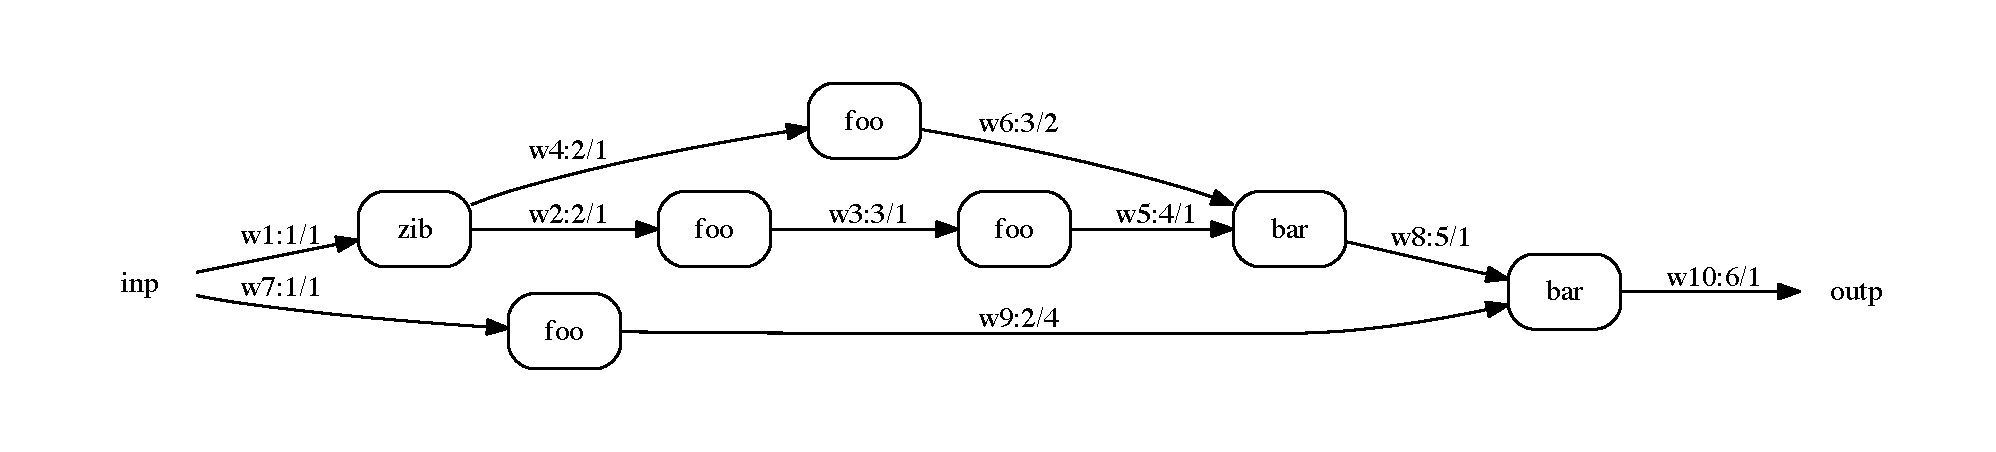
\includegraphics[width=\textwidth]{figs/sdf-fifosizes-ex}
  \caption{The dataflow graph generated by the CAPH compiler from the program in
    Listing.~\ref{lst:sdf-fifosizes-ex}, with edges annotated with the infered phase and FIFO size information}
  \label{fig:sdf-fifosizes-dfg}
\end{figure}
%%% Local Variables: 
%%% mode: latex
%%% TeX-master: "caph-lrm"
%%% End: 
